% Revised captions for the existing figures. No plotted data, smoothing,
% paths, or labels have been changed.
% Keep these floats near Section~\ref{sec:gd-experiments}. The first two
% figures should be discussed together because their diagnostics are linked.

\begin{figure*}[!t]
  \centering
  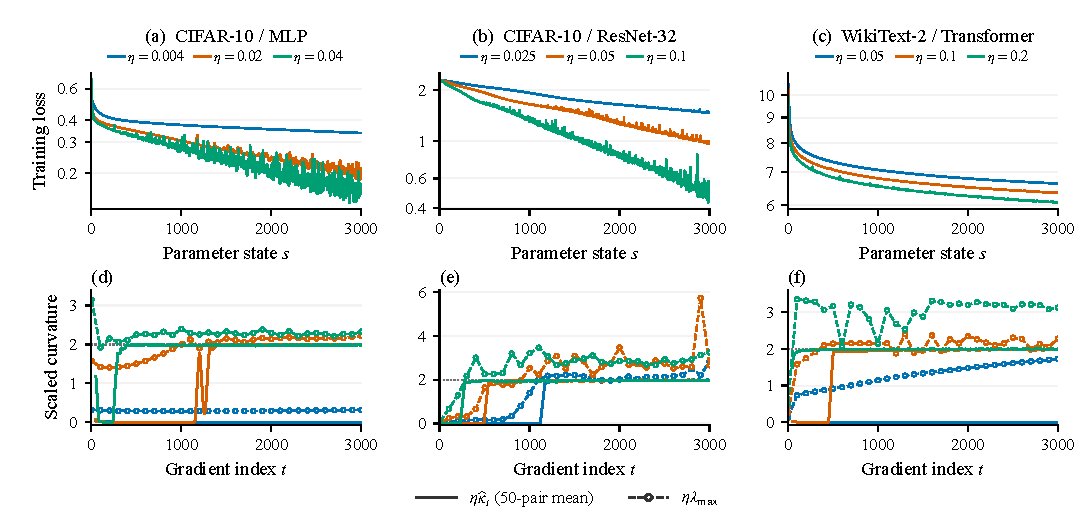
\includegraphics[width=\textwidth]{figures/analysis024/gd_loss_projected_change_spectral_clean.pdf}
  \caption{\textbf{Oscillatory loss reduction and directional curvature
  under full-batch GD.}
  Columns identify dataset/model; colors identify learning rate.
  Top: unsmoothed full-objective loss on logarithmic axes.
  Bottom: $\eta\widehat\kappa_t$ (solid, complete 50-pair trailing means)
  and recorded $\eta\lambda_{\max}$ measurements (dashed with circles).
  The dotted line at two is the quadratic-model loss-change threshold.
  The secant statistic averages directional curvature along a step;
  the spectral measurements are pointwise maxima and provide context.
  Spectra use the complete MLP objective, 5,000/50,000 ResNet images,
  and 2,500/59,680 Transformer sequences.
  Loss uses parameter state $s$; a spectrum at state $s$ is placed at
  gradient index $t=s+2$, the starting state for $\widehat\kappa_t$.
  The final spectrum has no recorded gradient pair.}
  \label{fig:gd-loss}
\end{figure*}

\begin{figure*}[!t]
  \centering
  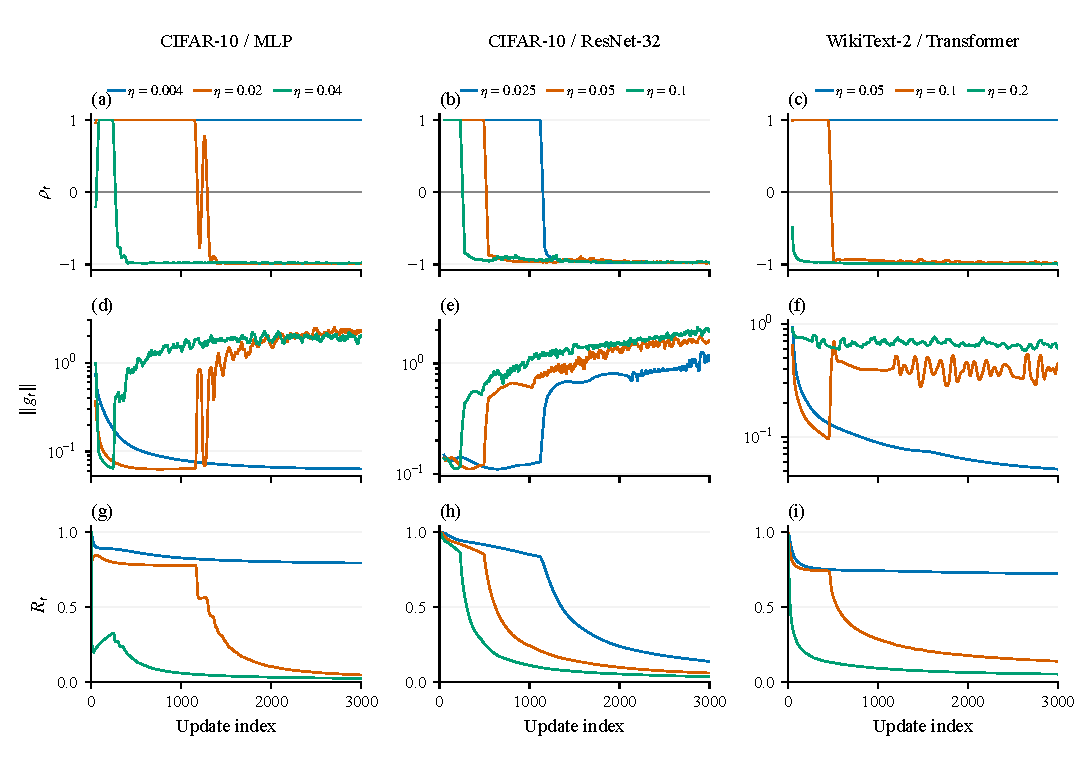
\includegraphics[width=\textwidth]{figures/analysis024/gd_reversal_norm_retention.pdf}
  \caption{\textbf{Strong consecutive reversal coexists with low final
  training loss.}
  Rows show consecutive gradient cosine, gradient norm (logarithmic scale),
  and normalized displacement $R_t$ for the conditions in
  Fig.~\ref{fig:gd-loss}. Cosines and norms use complete 50-observation
  trailing means; $R_t$ is the unsmoothed net-displacement-to-path-length
  ratio over the prefix through update $t$.
  At the largest tested rates, $R_{3000}$ is approximately 2.6\%, 3.7\%,
  and 5.4\% for the MLP, ResNet, and Transformer, respectively; each of
  these runs also attains its model's lowest final loss within the sweep.
  Negative cosine establishes local reversal; the path ratio describes
  cumulative geometry. Colors and column ordering match
  Fig.~\ref{fig:gd-loss}.}
  \label{fig:gd-alignment-displacement}
\end{figure*}

\begin{figure*}[!t]
  \centering
  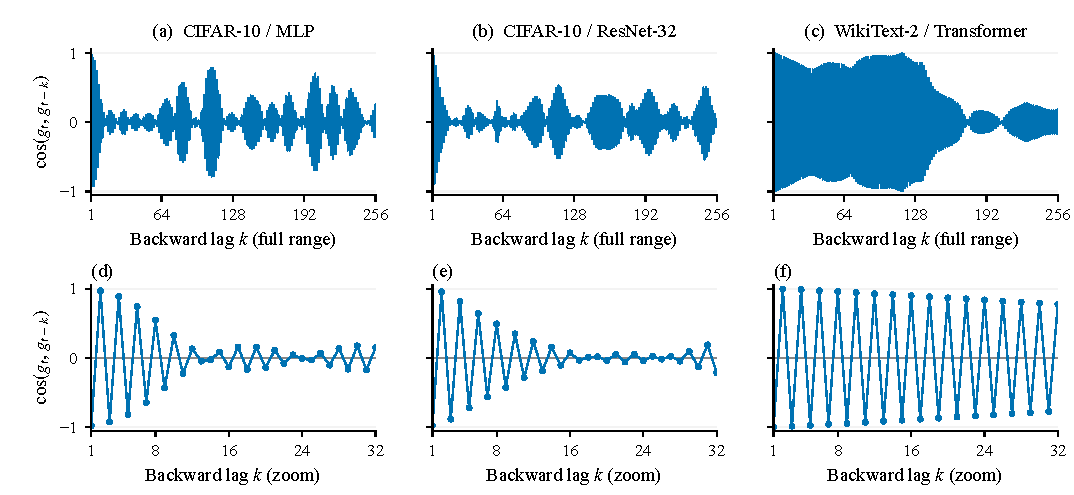
\includegraphics[width=\textwidth]{figures/analysis035/gd_backward_compact.pdf}
  \caption{\textbf{Odd--even lag alignment reveals recurring reversal.}
  Backward gradient alignment at the common endpoint $\theta_{2256}$,
  corresponding to $t=2257$. Each point is one exact
  $\cos(g_t,g_{t-k})$ with the endpoint fixed.
  Top: lags 1--256. Bottom: the same values at lags 1--32.
  Rates are $0.04$ (MLP), $0.1$ (ResNet), and $0.2$ (Transformer).
  These separately recomputed 256-update GD continuations start from
  recorded state 2000, with one initialization, no smoothing, and no
  endpoint averaging. The correlations describe temporal organization
  at this endpoint; net movement also depends on the gradient norms.}
  \label{fig:gd-backward}
\end{figure*}

\begin{figure*}[!t]
  \centering
  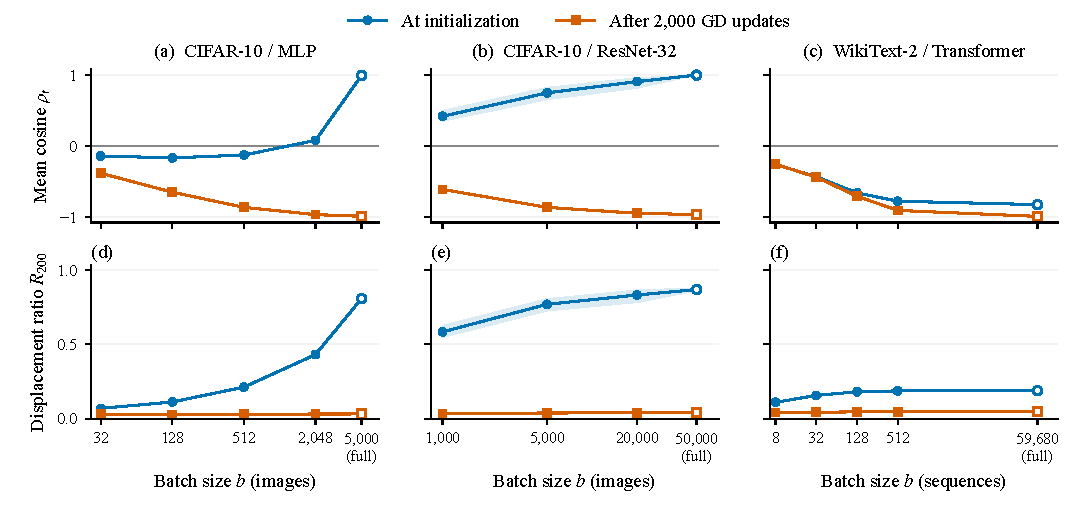
\includegraphics[width=\textwidth]{figures/analysis037/sgd_batch_size_compact.pdf}
  \caption{\textbf{Batch-size dependence of sampled-gradient alignment
  along SGD continuations.}
  Mean sampled-gradient cosine over 199 adjacent pairs during
  200-update continuations. Blue circles start at initialization;
  orange squares start after 2,000 GD updates. Each line averages
  repetitions within initialization, then weights the three
  initialization blocks equally; shading is their range, not a
  confidence interval. Hollow rightmost markers denote full GD.
  ResNet batches contain whole fixed 1,000-image normalization groups;
  Transformer batches count prepared sequences. Batch axes are logarithmic.
  Because the continuations update the parameters, the comparison includes
  both gradient sampling variability and changes in the visited states.}
  \label{fig:sgd-moving-geometry}
\end{figure*}
